\documentclass[journal]{vgtc}                % final (journal style)
%\documentclass[review,journal]{vgtc}         % review (journal style)
%\documentclass[widereview]{vgtc}             % wide-spaced review
%\documentclass[preprint,journal]{vgtc}       % preprint (journal style)
%\documentclass[electronic,journal]{vgtc}     % electronic version, journal

%% Uncomment one of the lines above depending on where your paper is
%% in the conference process. ``review'' and ``widereview'' are for review
%% submission, ``preprint'' is for pre-publication, and the final version
%% doesn't use a specific qualifier. Further, ``electronic'' includes
%% hyperreferences for more convenient online viewing.

%% Please use one of the ``review'' options in combination with the
%% assigned online id (see below) ONLY if your paper uses a double blind
%% review process. Some conferences, like IEEE Vis and InfoVis, have NOT
%% in the past.

%% Please note that the use of figures other than the optional teaser is not permitted on the first page
%% of the journal version.  Figures should begin on the second page and be
%% in CMYK or Grey scale format, otherwise, colour shifting may occur
%% during the printing process.  Papers submitted with figures other than the optional teaser on the
%% first page will be refused.

%% These three lines bring in essential packages: ``mathptmx'' for Type 1
%% typefaces, ``graphicx'' for inclusion of EPS figures. and ``times''
%% for proper handling of the times font family.

\usepackage{mathptmx}
\usepackage{graphicx}
\usepackage{times}

%% We encourage the use of mathptmx for consistent usage of times font
%% throughout the proceedings. However, if you encounter conflicts
%% with other math-related packages, you may want to disable it.

%% This turns references into clickable hyperlinks.
\usepackage[bookmarks,backref=true,linkcolor=black]{hyperref} %,colorlinks
\hypersetup{
  pdfauthor = {},
  pdftitle = {},
  pdfsubject = {},
  pdfkeywords = {},
  colorlinks=true,
  linkcolor= black,
  citecolor= black,
  pageanchor=true,
  urlcolor = black,
  plainpages = false,
  linktocpage
}

%% If you are submitting a paper to a conference for review with a double
%% blind reviewing process, please replace the value ``0'' below with your
%% OnlineID. Otherwise, you may safely leave it at ``0''.
\onlineid{0}

%% declare the category of your paper, only shown in review mode
\vgtccategory{Research}

%% allow for this line if you want the electronic option to work properly
\vgtcinsertpkg

%% In preprint mode you may define your own headline.
%\preprinttext{To appear in an IEEE VGTC sponsored conference.}

%% Paper title.

\title{MetroViz: Visual Analysis of Public Transportation Data}

%% This is how authors are specified in the journal style

%% indicate IEEE Member or Student Member in form indicated below
\author{Fan Du ...}
\authorfooter{
%% insert punctuation at end of each item
\item
 Fan Du is with University of Maryland, College Park. E-mail: fan@cs.umd.edu.
\item
 Ed Grimley is with Grimley Widgets, Inc.. E-mail: ed.grimley@aol.com.
\item
 Martha Stewart is with Martha Stewart Enterprises at Microsoft
 Research. E-mail: martha.stewart@marthastewart.com.
}

%other entries to be set up for journal
\shortauthortitle{Biv \MakeLowercase{\textit{et al.}}: Global Illumination for Fun and Profit}
%\shortauthortitle{Firstauthor \MakeLowercase{\textit{et al.}}: Paper Title}

%% Abstract section.
\abstract{
Motivation\\
Public transportation, including buses and rail lines, is an important resource for urban residents. Knowing how well the public transportation is serving the public is important for schedule optimization and resources allocation. Ridership and adherence are two main dimensions for evaluating the level-of-service (LOS)~\cite{camus2005estimation,hammerle2005use}.
% \\\\
% Problem statement\\
% Experts at the Department of Transportation need effective tools to aid exploring the data.
\\\\
Approach\\
Using the technology of Automatic Vehicle Location (AVL), Automatic Passenger Count (APC) and Global Positioning System (GPS), ridership data and adherence data of public transportation have been collected. In this paper, we developed a visualization system for exploring public transportation data. We designed a map view for exploring stops and routes, and a calender view for exploring ridership and adherence information of trips over years.
\\\\
Results\\
In the first round of usability testing, two researchers from the Center For Advanced Transportation Technology (CATT), and six Computer Science PhD students from the University of Maryland took part in a study in which they used our system to explore the bus transit data of Blacksburg, Virgina. The participants were able to use our system to explore bus stops, bus routes and ridership and adherence of bus trips.
\\\\
Conclusions\\
TODO

% Conclusions
%   Public transportation is an important part our daily life. In the operation of public transportation, ridership and adherence data have been collected. With the growth of data scale, the department of transportation is in need of powerful visualization tools to explore the data, and gain insights. In this paper, we developed a visual tool to help explore the data, and gain insights. Our tool provides a map view and a route view to help people quickly locate stops and routes. A calendar view to provide a overview of adherence / ridership information for several years. A trip and a stop view to help people get details of trips and stops on specific days. Two CATT Lab researchers and twelve computer science PhD students took part in a study in which they used our tool to explore bus ridership and adherence data of Blacksburg City. THe participants were able to use our tool to locate stops and routes, and detect abnormal stops and routes, and find abnormal days.
} % end of abstract

%% Keywords that describe your work. Will show as 'Index Terms' in journal
%% please capitalize first letter and insert punctuation after last keyword
\keywords{Public transportation, visual analysis}

%% ACM Computing Classification System (CCS). 
%% See <http://www.acm.org/class/1998/> for details.
%% The ``\CCScat'' command takes four arguments.

\CCScatlist{ % not used in journal version
 \CCScat{K.6.1}{Management of Computing and Information Systems}%
{Project and People Management}{Life Cycle};
 \CCScat{K.7.m}{The Computing Profession}{Miscellaneous}{Ethics}
}

%% Uncomment below to include a teaser figure.
  \teaser{
  \centering
  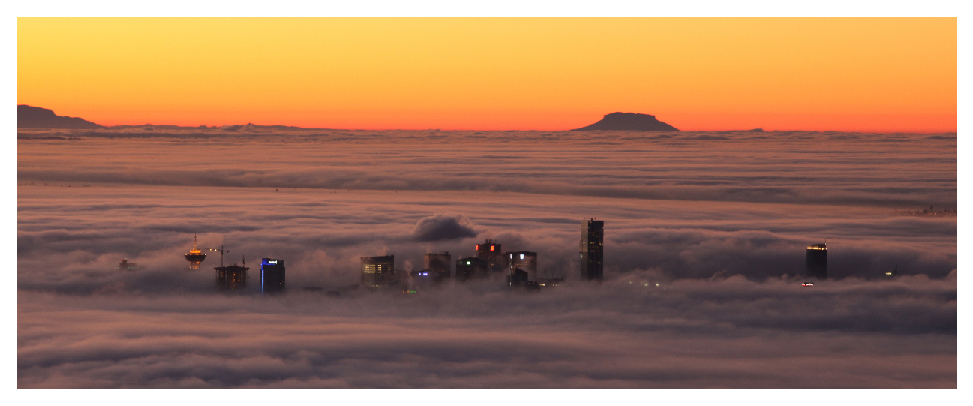
\includegraphics[width=16cm]{CypressView}
  \caption{In the Clouds: Vancouver from Cypress Mountain.}
  }

%% Uncomment below to disable the manuscript note
%\renewcommand{\manuscriptnotetxt}{}

%% Copyright space is enabled by default as required by guidelines.
%% It is disabled by the 'review' option or via the following command:
% \nocopyrightspace

%%%%%%%%%%%%%%%%%%%%%%%%%%%%%%%%%%%%%%%%%%%%%%%%%%%%%%%%%%%%%%%%
%%%%%%%%%%%%%%%%%%%%%% START OF THE PAPER %%%%%%%%%%%%%%%%%%%%%%
%%%%%%%%%%%%%%%%%%%%%%%%%%%%%%%%%%%%%%%%%%%%%%%%%%%%%%%%%%%%%%%%%

\begin{document}

%% The ``\maketitle'' command must be the first command after the
%% ``\begin{document}'' command. It prepares and prints the title block.

%% the only exception to this rule is the \firstsection command
\firstsection{Introduction}

\maketitle

%% \section{Introduction} %for journal use above \firstsection{..} instead

TODO: Fan

\section{Related Works}
Analyzing Automatic Vehicle Location (AVL) and Automatic Passenger Count (APC) Data
\\\\
Rancic et al.~\cite{Rancic2008} present a tracking system using AVL data to analyzing city bus transit traffic.
Chen \cite{5203406} introduces a model to simulate bus operation and passenger demand based on AVL and APC data.
\\\\
Travel Time Predicting
\\\\
Lee et al.~\cite{Lee:2012:HNF:2424321.2424357} introduce a real-time travel time prediction method based on multiple samples of similar historical trajectory.
Tiesyte and Jensen~\cite{Tiesyte2008} propose a method to predict the future movement of a vehicle based on the identification of the most similar historical trajectory.
Predic et al.~\cite{Predic2007} use real-time AVL data and historical data to predict bus motion and bus arrival time.
\\\\
Route Choosing
\\\\
Nguyen et al.~\cite{Nguyen2012} consider buses as moving objects, and use temporal maps to represent the movements of buses in spatio-temporal domain to help passengers choose approatiate routes.
Liu et al.~\cite{5958130} propose a bus trip planning system to help passengers choose the most appropriate lines and transfers, based on traffic data.
\\\\
Trajectory Visualization
\\\\
Tominski et al.~\cite{Tominski2012} use a hybrid 2D/3D display to show the trajectories and associated attributes in their spatial-temporal context.
Scheepens et al.~\cite{6065019} improve density maps to help explore trajectories using multiple density fields.
\\\\
Flows Visualization
\\\\
Guo~\cite{5290710} develops a visualization framework to interactively explore large-scale spatial flows.
Cui et al.~\cite{4658140} propose an edge-clustering method to reduce edge crossings and visualize geometry graphs.
\\\\
Improving Bus Scheduling
\\\\
Kimpel et al.~\cite{4658140} discuss efforts of using the TriMet [*] APC and AVL data to improve buses scheduling.
Yu and Yang~\cite{Yu2007} develop a dynamic holding strategy to optimize the holding strategy.
\\\\
Schedule Adherence
\\\\
Mai et al.~\cite{mai2011visualizing} extend the Marey graph by adding schedule adherence and passenger load information to measure transit performance.
\\\\
Level-of-Service (LOS) Estimation
\\\\
Camus et al.~\cite{camus2005estimation} propose a way to estimation the level-of-service (LOS) based on AVL data.
Hammerle et al.~\cite{hammerle2005use} analyze the AVL and APC data of Chicago Transit Authority to estimate service reliability.
\\\\
Maps on Mobile Device
\\\\
Wang and Chi~\cite{6065020} introduce a focus+context method to visualize metro map on small displaying area of mobile devices.
\\\\
Public Transit Services
\\\\
Wmata [*]: Washington Metropolitan Area Transit Authority.
TriMet [*]: Public Transit in the Portland Area.
BT [*]: Blacksburg Transit provides bus transportation primarily to and from the campus of Virginia Tech.

\section{System Overview}
TODO: Peter

\section{Data Processing}
TODO: Yoav

\section{Visual Design}
\subsubsection{Map View}
TODO: Fan
\subsubsection{Route View}
TODO: Varun
\subsubsection{Calender View}
TODO: Peter
\subsubsection{Trip View}
TODO: Peter
\subsubsection{Stop View}
TODO: Josh

\section{Evaluation}
\subsubsection{Methodology}
TODO: Varun
\subsubsection{Results}
TODO: Josh

\section{Discussion and Future Work}
TODO: Peter

\section{Credits}

\paragraph{Rejected Ejector Seat Reservation}

%% if specified like this the section will be committed in review mode
\acknowledgments{
The authors wish to thank A, B, C. This work was supported in part by
a grant from XYZ.}

\bibliographystyle{abbrv}
%%use following if all content of bibtex file should be shown
%\nocite{*}
\bibliography{template}
\end{document}
